\section{Computation}

\begin{frame}{1-D discrete case}
    \footnotesize
    Here $\mX=\mY=\R$. Suppose
     $\alpha=\frac{1}{n}\sum_{i=1}^n \delta_{x_i}$
    and $\beta=\frac{1}{n}\sum_{i=1}^n \delta_{y_i}$
    where $x_1\leq \cdots \leq x_n$ and $y_1\leq \cdots \leq y_n$.

    \begin{figure}
        \centering
        \captionsetup{font=scriptsize}
        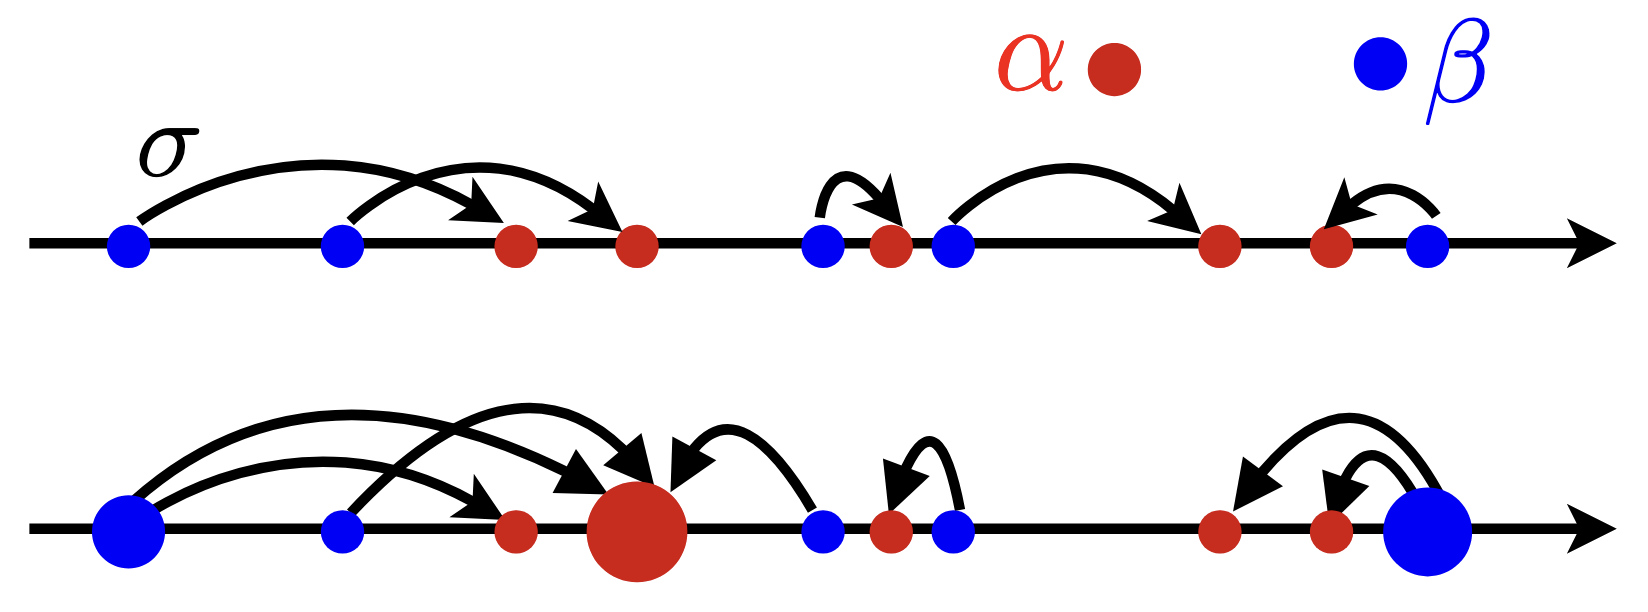
\includegraphics[width=0.5\textwidth]{png/1d-discrete.png}
        \caption{1-D optimal transport in discrete case}
    \end{figure}
    
    Then the $p$-Wasserstein distance can be simply computed by
    \begin{equation}
        \wass_p(\alpha,\beta)^p = \frac{1}{n}\sum_{i=1}^n |x_i-y_i|^p.
    \end{equation}
    It's in fact a greedy algorithm.
\end{frame}

\begin{frame}{1-D continuous case}
    \footnotesize
    \vspace{-.5em}
    If $\mu,\nu$ are 1-D measures with densities. Suppose their 
    cummulative distribution functions are $\mathcal{C}_\mu$ and $\mathcal{C}_\nu$, respectively.
    Then the $\wass_1$ distance could be computed by
    \begin{equation}
        \wass_1(\mu,\nu) = \int_\R |\mathcal{C}_\mu(x)-\mathcal{C}_\nu(x)|\;dx
        = \int_\R \left|\int_{-\infty}^x d(\mu-\nu)\right|\; dx.
    \end{equation}
    And the Monge map is then defined by
    \begin{equation}
        T = \mathcal{C}_\nu^{-1}\circ \mathcal{C}_\mu.
    \end{equation}
    \begin{figure}
        \captionsetup{font=scriptsize}
        \begin{minipage}[c]{0.32\linewidth}
            \vspace{0pt}
            \centering
            \includegraphics[width=0.85\textwidth]{png/1d-continuous/mu.epsc}
            \caption*{$\mu$}
        \end{minipage}
        \hfill
        \begin{minipage}[c]{0.32\linewidth}
            \vspace{0pt}
            \centering
            \includegraphics[width=0.85\textwidth]{png/1d-continuous/nu.epsc}
            \caption*{$\nu$}
        \end{minipage}
        \hfill
        \begin{minipage}[c]{0.32\linewidth}
            \vspace{0pt}
            \centering
            \includegraphics[width=0.85\textwidth]{png/1d-continuous/transfer.epsc}
            \caption*{$(tT+(1-t)\text{Id})_\#\mu$}
        \end{minipage}
    \end{figure}

    \vspace{-1.2em}
    \begin{figure}
        \captionsetup{font=scriptsize}
        \begin{minipage}[c]{0.24\linewidth}
            \vspace{0pt}
            \centering
            \includegraphics[width=0.75\textwidth]{png/1d-continuous/CmuCnu.epsc}
            \caption*{$(\mathcal{C}_\mu,\mathcal{C}_\nu)$}
        \end{minipage}
        \hfill
        \begin{minipage}[c]{0.24\linewidth}
            \vspace{0pt}
            \centering
            \includegraphics[width=0.75\textwidth]{png/1d-continuous/CinvmuCinvnu.epsc}
            \caption*{$(\mathcal{C}^{-1}_\mu,\mathcal{C}^{-1}_\nu)$}
        \end{minipage}
        \hfill
        \begin{minipage}[c]{0.24\linewidth}
            \vspace{0pt}
            \centering
            \includegraphics[width=0.75\textwidth]{png/1d-continuous/TTinv.epsc}
            \caption*{$(T,T^{-1})$}
        \end{minipage}
        \hfill
        \begin{minipage}[c]{0.24\linewidth}
            \vspace{0pt}
            \centering
            \includegraphics[width=0.75\textwidth]{png/1d-continuous/Cinvtrans.epsc}
            \caption*{$(1-t)\mathcal{C}^{-1}_\mu+t\mathcal{C}^{-1}_\nu$}
        \end{minipage}

        \vspace{-1em}
        \caption{Computation of OT and displacement interpolation between two 1-D measures.}
    \end{figure}
    
\end{frame}

\begin{frame}{1-D Gaussian}
    \footnotesize
    If $\mu=\mathcal{N}(m_1,\sigma_1^2),\nu=\mathcal{N}(m_2,\sigma_2^2)$ are 1-D Gaussians.
    Then the $\wass_2$ distance can be directly computed by
    \begin{equation}
        \wass_2(\mu,\nu) = \sqrt{|m_1-m_2|^2 + |\sigma_1-\sigma_2|^2},
    \end{equation}
    which is thus the Euclidean distance on the 2-D plane 
    plotting the mean and the standard deviation of a Gaussian $\mathcal{N}(m, \sigma)$.

    \begin{figure}
        \captionsetup{font=scriptsize}
        \begin{minipage}[c]{0.48\linewidth}
            \vspace{0pt}
            \centering
            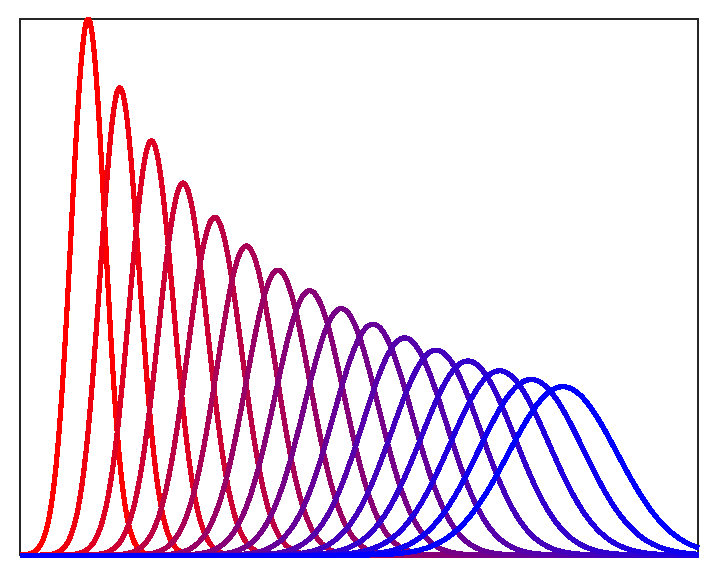
\includegraphics[width=0.85\textwidth]{png/1d-gaussian/interp-density.eps}
        \end{minipage}
        \hfill
        \begin{minipage}[c]{0.48\linewidth}
            \vspace{0pt}
            \centering
            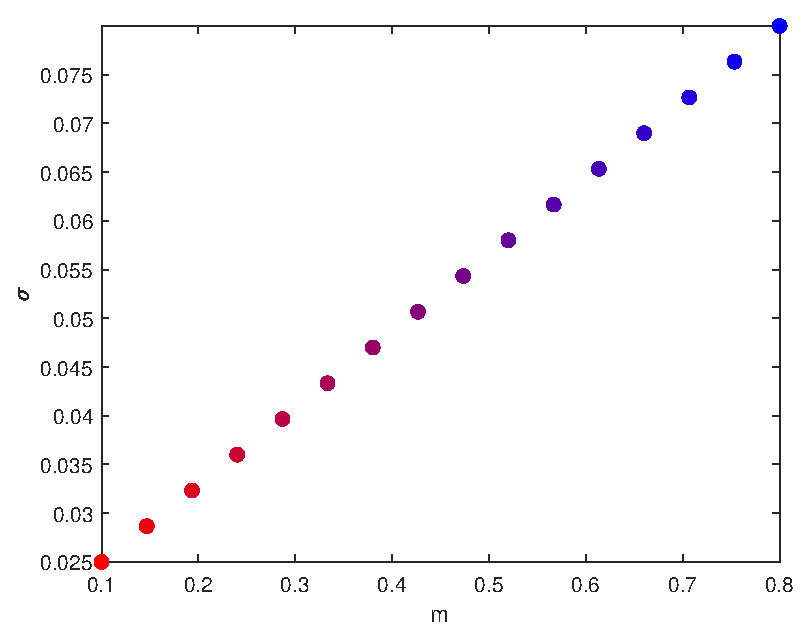
\includegraphics[width=0.85\textwidth]{png/1d-gaussian/plane.eps}
        \end{minipage}
        \caption{Computation of displacement interpolation between two 1-D Gaussians.}
    \end{figure}

    \vspace{-1em}
    Learn more in [Takatsu, 2011]\footfullcite{Takatsu2011}.
\end{frame}

\begin{frame}{Discretization}
    \footnotesize
    Suppose $\mu$ is a measure with density $\rho$, supported on $[0,1]$.
    Let
    \begin{equation}
        \tilde\mu = \sum_{i=0}^N u_i \delta_{x_i}, 
    \end{equation}
    where
    \begin{equation}
        u_i = \frac{\rho(x_i)}{N+1},\quad x_i=\frac{i}{N},\quad i=0,...,N.
    \end{equation}
    We call $\tilde\mu$ the \textit{discretization} of $\mu$.
    This technique can also be used in $\R^d$.
    
    \pause\vspace{1em}
    Let $\tilde\nu = \sum_{i=0}^M v_i \delta_{y_i}$ 
    and $(\vect{C})_{ij}$ be the cost matrix.
    The Kantorovich problem then becomes
    \begin{equation}
        L_{\vect C}(\vect u,\vect v) := \min_{\vect P\in U(\vect u, \vect v)} \langle \vect P, \vect C \rangle
        := \min_{\vect P\in U(\vect u, \vect v)} \sum_{i,j} \vect{P}_{ij} \vect{C}_{ij},
    \end{equation}
    where
    \begin{equation}
        U(\vect u,\vect v) := \left\{ \vect P \left| 
        \sum_{j} \vect{P}_{ij} = u_i,\forall i,\quad \text{and}\quad
        \sum_{i} \vect{P}_{ij} = v_j,\forall j
        \right.
        \right\}.
    \end{equation}
\end{frame}

\begin{frame}{Entropy regularization}
    \footnotesize
    Define the entropy
    \begin{equation}
        H(\vect P) := -\sum_{i,j} \vect{P}_{ij}(\log(\vect{P}_{ij})-1).
    \end{equation}
    Then the regularized Kantorovich problem\footfullcite{Wilson1969} is defined by
    \begin{equation}
        L_{\vect C}^\varepsilon (\vect u,\vect v)
        := \min_{\vect P\in U(\vect u, \vect v)} 
        \langle \vect P, \vect C \rangle - \varepsilon H(\vect P).
    \end{equation}
    It can be shown that
    $L_{\vect C}^\varepsilon (\vect u,\vect v)
        = L_{\vect C} (\vect u,\vect v) + O(\varepsilon)$.

    \begin{figure}
        \captionsetup{font=scriptsize}
        \begin{minipage}[t]{0.05\linewidth}
            \vspace{0pt}
            \hfill
        \end{minipage}
        \hfill
        \begin{minipage}[t]{0.18\linewidth}
            \vspace{0pt}
            \centering
            \includegraphics[width=0.95\textwidth]{png/entropy-regularization/mu.epsc}
        \end{minipage}
        \hfill
        \begin{minipage}[t]{0.18\linewidth}
            \vspace{0pt}
            \hfill
        \end{minipage}
        \hfill
        \begin{minipage}[t]{0.18\linewidth}
            \vspace{0pt}
            \hfill
        \end{minipage}
        \hfill
        \begin{minipage}[t]{0.18\linewidth}
            \vspace{0pt}
            \hfill
        \end{minipage}
        \hfill
        \begin{minipage}[t]{0.18\linewidth}
            \vspace{0pt}
            \hfill
        \end{minipage}
        \hfill
    \end{figure}
    
    \vspace{-1em}
    \begin{figure}
        \captionsetup{font=scriptsize}
        \begin{minipage}[t]{0.05\linewidth}
            \vspace{0pt}
            \centering
            \includegraphics[width=0.88\textwidth]{png/entropy-regularization/nu.epsc}
        \end{minipage}
        \hfill
        \begin{minipage}[t]{0.18\linewidth}
            \vspace{0pt}
            \centering
            \includegraphics[width=0.95\textwidth]{png/entropy-regularization/EntroRegu1.epsc}
            \caption*{$\varepsilon = 1$}
        \end{minipage}
        \hfill
        \begin{minipage}[t]{0.18\linewidth}
            \vspace{0pt}
            \centering
            \includegraphics[width=0.95\textwidth]{png/entropy-regularization/EntroRegu2.epsc}
            \caption*{$\varepsilon = 5\times 10^{-2}$}
        \end{minipage}
        \hfill
        \begin{minipage}[t]{0.18\linewidth}
            \vspace{0pt}
            \centering
            \includegraphics[width=0.95\textwidth]{png/entropy-regularization/EntroRegu3.epsc}
            \caption*{$\varepsilon = 10^{-2}$}
        \end{minipage}
        \hfill
        \begin{minipage}[t]{0.18\linewidth}
            \vspace{0pt}
            \centering
            \includegraphics[width=0.95\textwidth]{png/entropy-regularization/EntroRegu4.epsc}
            \caption*{$\varepsilon = 10^{-3}$}
        \end{minipage}
        \hfill
        \begin{minipage}[t]{0.18\linewidth}
            \vspace{0pt}
            \centering
            \includegraphics[width=0.95\textwidth]{png/entropy-regularization/EntroRegu5.epsc}
            \caption*{$\varepsilon = 10^{-4}$}
        \end{minipage}
        \hfill
        \vspace{-.8em}
        \caption{Graphs of optimal $\vect P$s when choose different $\varepsilon$. Set $\vect C_{ij} = |x_i-x_j|^2$.}
    \end{figure}
\end{frame}

\begin{frame}{Sinkhorn iteration}
    \footnotesize
    Let $\vect K_{ij} = e^{-\frac{\vect C_{ij}}{\varepsilon}}$.
    Sinkhorn iteration writes
    \begin{equation}
        \vect a^{(l+1)} \gets \frac{\vect u}{\vect K \vect b^{(l)}},
        \quad \text{and}\quad
        \vect b^{(l+1)} \gets \frac{\vect v}{\vect K^T \vect a^{(l+1)}},
        \quad \text{for}\; l=0,1,...
    \end{equation}
    which starts with an arbitary $\vect b^{(0)}$.
    The transport matrix $\vect P$ can be rebuilt by
    \begin{equation}
        \vect P^{(l)} = \text{diag}\left(\vect b^{(l)}\right)
        \cdot \vect K \cdot \text{diag}\left(\vect a^{(l)}\right).
    \end{equation}
    The convergence is proved by Sinkhorn\footfullcite{Sinkhorn1964}.
    And Altschuler et al\footfullcite{Altschuler2017} give an analysis of the computational complexity.

    \vspace{-1em}
    \begin{figure}
        \captionsetup{font=scriptsize}
        \begin{minipage}[t]{0.05\linewidth}
            \vspace{0pt}
            \hfill
        \end{minipage}
        \hfill
        \begin{minipage}[t]{0.18\linewidth}
            \vspace{0pt}
            \centering
            \includegraphics[width=0.95\textwidth]{png/entropy-regularization/mu.epsc}
        \end{minipage}
        \hfill
        \begin{minipage}[t]{0.18\linewidth}
            \vspace{0pt}
            \hfill
        \end{minipage}
        \hfill
        \begin{minipage}[t]{0.18\linewidth}
            \vspace{0pt}
            \hfill
        \end{minipage}
        \hfill
        \begin{minipage}[t]{0.18\linewidth}
            \vspace{0pt}
            \hfill
        \end{minipage}
        \hfill
        \begin{minipage}[t]{0.18\linewidth}
            \vspace{0pt}
            \hfill
        \end{minipage}
        \hfill
    \end{figure}
    
    \vspace{-1em}
    \begin{figure}
        \captionsetup{font=scriptsize}
        \begin{minipage}[t]{0.05\linewidth}
            \vspace{0pt}
            \centering
            \includegraphics[width=0.88\textwidth]{png/entropy-regularization/nu.epsc}
        \end{minipage}
        \hfill
        \begin{minipage}[t]{0.18\linewidth}
            \vspace{0pt}
            \centering
            \includegraphics[width=0.95\textwidth]{png/entropy-regularization/iter1.epsc}
            \caption*{$l = 1$}
        \end{minipage}
        \hfill
        \begin{minipage}[t]{0.18\linewidth}
            \vspace{0pt}
            \centering
            \includegraphics[width=0.95\textwidth]{png/entropy-regularization/iter10.epsc}
            \caption*{$l = 10$}
        \end{minipage}
        \hfill
        \begin{minipage}[t]{0.18\linewidth}
            \vspace{0pt}
            \centering
            \includegraphics[width=0.95\textwidth]{png/entropy-regularization/iter50.epsc}
            \caption*{$l = 50$}
        \end{minipage}
        \hfill
        \begin{minipage}[t]{0.18\linewidth}
            \vspace{0pt}
            \centering
            \includegraphics[width=0.95\textwidth]{png/entropy-regularization/iter100.epsc}
            \caption*{$l = 100$}
        \end{minipage}
        \hfill
        \begin{minipage}[t]{0.18\linewidth}
            \vspace{0pt}
            \centering
            \includegraphics[width=0.95\textwidth]{png/entropy-regularization/iter1000.epsc}
            \caption*{$l = 1000$}
        \end{minipage}
        \hfill
        \vspace{-1.2em}
        \caption{Graphs of $\vect P^{(l)}$. Set $\vect C_{ij} = |x_i-x_j|^2$ and $\varepsilon=10^{-3}$.}
    \end{figure}
\end{frame}